\documentclass[10pt]{article}
\usepackage{hyperref}
\usepackage{geometry}
\usepackage{graphicx}
\usepackage{slashed}
\usepackage{cite}
\usepackage{bbm}
\usepackage{dsfont}
\usepackage{color}
\geometry{a4paper,margin=20mm}
\usepackage{indentfirst}
\usepackage{multirow}
\usepackage{subfigure}
\usepackage{float}
\usepackage{makecell}
\usepackage{amsmath,amsfonts,amssymb}
\usepackage{tikz,pgf}
\usepackage{cleveref}
\usepackage{subcaption}
\usepackage{booktabs}
\usepackage[table]{xcolor} %给表格加颜色


\usetikzlibrary{calc}
%\usetikzlibrary{arrows.meta}
\usetikzlibrary{intersections}
\usetikzlibrary{trees}
\usetikzlibrary{decorations.pathmorphing}
\usetikzlibrary{decorations.markings}
\usetikzlibrary{patterns}
\tikzset{
   global scale/.style={
      scale=#1,
      every node/.append style={scale=#1}},
   photon/.style={decorate, decoration={snake}, draw=red},
   nucleon/.style={draw=black, postaction={decorate},
      decoration={markings,mark=at position .55 with{\arrow[draw=black]{>}}}},
   delta/.style={
      line width=2pt,
      double distance=1.5pt,
      draw=black,
      postaction={
        decorate},
        decoration={
          markings,
          mark=at position .55 with {\arrow[draw=black, scale=0.5]{>}}
        }
    },
   pion/.style={draw=blue, postaction={decorate},
      decoration={markings,mark=at position .55 with{\arrow[draw=blue]{}}}},
    }

\allowdisplaybreaks[4]


\begin{document}

\title{Differential Cross Sections for Electron-Proton Bremsstrahlung in Covariant Chiral Perturbation Theory at JLab Kinematics}

\author{Xu Wang \textsuperscript{1}\footnote{wangxu0604@stu.pku.edu.cn},
Kai-Ge Kang \textsuperscript{1}\footnote{kaige@alumni.pku.edu.cn},
Xiong-Hui Cao \textsuperscript{2}\footnote{xhcao@itp.ac.cn},
and Han-Qing Zheng \textsuperscript{3}\footnote{zhenghq@scu.edu.cn}\\
\small \textsuperscript{1} School of Physics, Peking University, Beijing 100871, China\\
\small \textsuperscript{2} Institute of Theoretical Physics, Chinese Academy of Sciences, Beijing 100190, China\\
\small \textsuperscript{3} Institute of Particle and Nuclear Physics, College of Physics, Sichuan University, Chengdu, Sichuan 610065, China
}
\maketitle

\begin{abstract}
This study presents a theoretical calculation of the scattering amplitude for the $ep\to ep\gamma$ process within the framework of Chiral Perturbation Theory (ChPT). We specifically focus on evaluating the tree-level Feynman diagrams up to $O(p^3)$ that contribute to this reaction. The process is of significant interest as it provides valuable insights into the generalized polarizabilities of the nucleon, which are fundamental properties characterizing its response to electromagnetic fields. Our calculations, based on the $O(p^2)$ and $O(p^3)$ nucleon-pion Lagrangians, aim to provide a theoretical prediction for the differential cross-section. By comparing our results with future experimental data, we seek to determine the values of the low-energy constants (LECs) and validate ChPT as an effective low-energy theory of QCD.
\end{abstract}

\section{Introduction}

Quantum Chromodynamics (QCD), the fundamental theory describing strong interactions, faces significant computational challenges in the low-energy regime due to non-perturbative effects. Chiral Perturbation Theory ($\chi$PT), as a low-energy effective field theory (EFT) of QCD, provides a rigorous framework to address these difficulties by preserving the essential features of chiral symmetry and its spontaneous breaking. Covariant Chiral Perturbation Theory, in particular, offers a systematic description of low-energy hadronic processes while maintaining Lorentz covariance and model independence. Developments in renormalization schemes, most notably the Extended-On-Mass-Shell (EOMS) scheme \cite{PhysRevD.68.056005}, have successfully resolved long-standing issues such as baryon magnetic moments \cite{PhysRevLett.101.222002} and proton Compton scattering \cite{Lensky_2009}. Furthermore, it exhibits superior convergence properties compared to Heavy Baryon Chiral Perturbation Theory ($\text{HB}\chi\text{PT}$) \cite{Martin_Camalich_2010}, providing a high-precision theoretical tool for low-energy strong interaction research.

The success of covariant $\chi$PT has been verified across several critical domains. In $\pi N$ scattering, $\text{B}\chi\text{PT}$ has laid the foundation for studying nucleon structure through the precise description of pion-proton interactions at low energies \cite{Alarc_n_2013,Chen_2013}. In photoproduction processes, partial wave analysis (PWA) based on covariant chiral theory has successfully elucidated the primary physical mechanisms underlying $\pi^+\pi^-$ photon production \cite{GomezTejedor1996}, with research indicating that the $f_0(980)$, $\rho(770)$, and $f_2(1270)$ mesons dominate the $S$-wave, $P$-wave, and $D$-wave contributions, respectively \cite{Battaglieri2009}. Regarding resonances, covariant chiral EFT not only accurately describes the properties of traditional vector resonances like the $\rho(770)$ \cite{Oller2000}, but also characterizes the dynamical structures of various decay channels in complex processes such as hyperon weak radiative decays (e.g., $\Lambda \to n\gamma$) \cite{Geng2009LambdaGamma}. These achievements provide a reliable theoretical benchmark for testing the Standard Model and exploring potential new physics effects.

Electron-proton ($ep$) elastic scattering remains a primary tool for probing the electromagnetic structure of the nucleon, supported by high-precision experimental data from world-class laboratories including BINP, CERN, DESY, Fermilab, JLab, MAMI, and SLAC. This data serves as the basis for extracting the proton's electromagnetic form factors, $G_E(Q^2)$ and $G_M(Q^2)$. Recently, interest in this field has intensified due to two major controversies: first, the discrepancy between $G_E/G_M$ ratios measured via polarization transfer versus the traditional Rosenbluth separation \cite{PERDRISAT2007694}; and second, the ``proton radius puzzle''---the unresolved inconsistency between the proton charge radius derived from muonic hydrogen Lamb shift experiments \cite{muonshift} and those from $ep$ scattering or electronic hydrogen spectroscopy \cite{RevModPhys.80.633,PhysRevLett.105.242001,annurev-nucl-102212-170627}. These mysteries have prompted new high-precision experiments at very low momentum transfer ($Q^2$), such as the PRad experiment at JLab \cite{Xiong:2019Nature}, COMPASS++/AMBER at CERN \cite{adams2019letterintentnewqcd,xiong2023protonchargeradiuslepton}, and MUSE at PSI \cite{gilman2013studyingprotonradiuspuzzle,gilman2017technicaldesignreportpaul}.

These experiments focus on the extremely low $Q^2$ region, placing stringent demands on theoretical accuracy. For instance, the MUSE experiment aims to measure $\mu p$ scattering cross-sections within $|Q^2| \sim 0.0016$--$0.08\ \text{GeV}^2$ to reach sub-percent precision on the charge radius, using lepton beams with momenta as low as $115$, $153$, and $210\ \text{MeV}$. At these scales, traditional radiative correction methods---such as the Mo-Tsai formula, the ultra-relativistic approximation ($E \gg m_e$) \cite{PhysRevC.62.054320}, or the Soft Photon Approximation (SPA) \cite{PhysRev.122.1898}---become inadequate. A central conflict arises between detector characteristics and traditional assumptions: the PRad experiment's Hybrid Calorimeter (HyCal) features a large acceptance and high energy resolution capable of detecting MeV-level photons \cite{Xiong:2019Nature}. In contrast, the SPA assumes photon energies are far below detector thresholds, often neglecting actual detector response functions in favor of a simple ``hard cutoff'' assumption. This leads to systematic biases in calculating real photon contributions. Furthermore, for $\mu p$ scattering, the muon mass ($m_\mu \approx 105.7\ \text{MeV}$) is non-negligible, rendering the ultra-relativistic approximation entirely invalid.

The precise description of real photon emission is the decisive factor in the accuracy of radiative corrections, particularly for the three-body final state process $ep \to ep\gamma$. This process encompasses the Bethe-Heitler (BH) mechanism, Virtual Compton Scattering (VCS), and their interference. The photon's angular and energy distributions, relative to detector acceptance, directly impact the reliability of extracting $G_E(Q^2)$, $G_M(Q^2)$, and the proton radius. Consequently, a systematic theoretical study of $ep \to ep\gamma$ is not only essential for refining radiative corrections at very low $Q^2$ but is also a prerequisite for resolving the proton structure puzzles. Only through an accurate description of differential cross-sections and phase space can real photon contributions be reliably separated from experimental data, ensuring the correct isolation of elastic scattering signals.

In this work, we first present the Lagrangians and Feynman rules required for the $ep \to ep\gamma$ process. Based on these rules, we calculate the $\mathcal{O}(p^3)$ tree-level amplitudes for both the BH and VCS processes to obtain the total scattering amplitude. Utilizing data from JLab E00-110 experiment\cite{defurne2015e00}, we perform a fit of the low-energy constants (LECs) appearing in the covariant chiral framework. Finally, we provide a concise and efficient method for calculating differential cross-sections---specifically designed for $\mu p$ scattering (where lepton mass is significant) and future hard-photon scattering studies---and provide theoretical predictions using our fitted LECs alongside those calculated by Fuchs et al. \cite{fuchs2004electromagnetic}.


\section{Theoretical formalism}








\subsection{Chiral Perturbation Theory}
Chiral Perturbation Theory (ChPT) is the low-energy effective field theory of QCD that describes the interactions of mesons and nucleons. The results of calculations in ChPT are expanded in terms of a small parameter, $p/(4\pi F)$, where $p$ represents the meson mass or external momentum, and $F$ is the meson decay constant in the chiral limit, with $4\pi F \sim 1 \text{GeV}$. The Lagrangian in ChPT is also constructed order by order based on this small parameter. In the process of calculating the $ep \to ep\gamma$ process, we need to use the $\mathcal{O}(p^3)$ Lagrangians, $\mathcal{L}_{\pi N}^{(2)}$ and $\mathcal{L}_{\pi N}^{(3)}$.


First, we give the Lagrangians up to $O(p^3)$ \cite{fettes2000chiral}:
\begin{align}
      \begin{aligned}
      \mathcal{L}_{\pi N}^{(1)}&=\bar{\Psi}\Bigl(
         i\slashed{D}-m+\frac{g_A}{2}\slashed{u}\gamma_5
      \Bigr)\Psi,\\
      \mathcal{L}_{\pi N}^{(2)}&=c_1 \langle \chi_+\rangle + \bar{\Psi}\sigma^{\mu\nu}[\frac{c_6}{8m}F_{\mu\nu}^+ + \frac{c_7}{8m}\langle F_{\mu\nu}^{+}\rangle]\Psi,\footnotemark
      \\
      \mathcal{L}_{\pi N}^{(3)}&= \bar{\Psi} \Bigl(\frac{d_6}{2 m} i\left[D^\mu, \widetilde{F}_{\mu \nu}^{+}\right] D^\nu+ \text{h.c.}\Bigr) \Psi + \bar{\Psi} \Bigl(\frac{d_7}{2 m} i\left[D^\mu,\left\langle F_{\mu \nu}^{+}\right\rangle\right] D^\nu+ \text{h.c.}\Bigr) \Psi,
      \end{aligned}
\end{align}
\footnotetext{The definitions of the $c_6$ and $c_7$ terms used here differ slightly from those in Scherer's work \cite{scherer2005}. The relationship between the two sets of coefficients is $c_6=4m_N c_6^{\prime}$, $c_7=m_N(-2c_6^{\prime}+c_7^{\prime})$.\label{lecs_footnote}}
where some terms are defined as follows:$D_{\mu}\Psi=\Bigl(\partial_{\mu}+\Gamma_{\mu}\Bigr)\Psi$, and
\begin{align}
   \begin{aligned}
  \Gamma_{\mu}&=\frac{1}{2}[u^{\dagger}(\partial_{\mu}-ir_{\mu})u+u(\partial_{\mu}-il_{\mu})u^{\dagger}],\\
u^{\mu}&=i[u^{\dagger}(\partial_{\mu}-ir_{\mu})u-u(\partial_{\mu}-il_{\mu})u^{\dagger}],\\
\chi_{\pm}&=u^{\dagger}\chi u^{\dagger}\pm u\chi^{\pm}u,\\
F_{\mu\nu}^{\pm}&=uF_{L\mu\nu}u^{\dagger}\pm u^{\dagger}F_{R\mu\nu}u,\\
F_{L,\mu\nu}&=\partial_{\mu}l_{\nu}-\partial_{\nu}l_{\mu}-i[l_{\mu},l_{\nu}],\\
F_{R,\mu\nu}&=\partial_{\mu}r_{\nu}-\partial_{\nu}r_{\mu}-i[r_{\mu},r_{\nu}].
\end{aligned}
\end{align}
Here, the symbols denote the following: $\langle X \rangle$ represents the trace, $\tilde{X} = X - \frac{1}{2} \langle X \rangle$, and h.c. stands for Hermitian conjugate.

Some common terms in the Lagrangian, after expanding the meson fields, are as follows:
\begin{align}
   \begin{aligned}
      &u = \mathbbm{1} + i\frac{\phi}{2F} -\frac{\phi^2}{8F^2} + \mathcal{O}(\phi^3),\\
      &\Gamma_{\mu} = -ir_{\mu} + \frac{1}{8F^2}[\phi \partial_{\mu}\phi - (\partial_{\mu}\phi)\phi] - \frac{i}{4F^2}\phi r_{\mu}\phi +\frac{i}{8F^2}\phi^2 r_{\mu} + \frac{i}{8F^2}r_{\mu}\phi^2 + \mathcal{O}(\phi^3),
      \\
      &u_{\mu} = -\frac{1}{F}\partial_{\mu}\phi + \frac{i}{F}r_{\mu}\phi -\frac{i}{F}\phi r_{\mu} + \mathcal{O}(\phi^3),\\
      &\chi_{+} = 2M^2\mathbbm{1} - \frac{1}{F^2}M^2\phi^2 + \mathcal{O}(\phi^3),\\
      &\chi_{-}=-\frac{2i}{F}M^2\phi^2 + \mathcal{O}(\phi^3),\\
      &F_{L,\mu\nu}=F_{R,\mu\nu}=-eF_{\mu\nu}Q,\\
      &F_{\mu\nu}^{+} = 2F_{R,\mu\nu} + \frac{1}{2F^2}\phi F_{R,\mu\nu}\phi -\frac{1}{4F^2}\phi^2F_{R,\mu\nu}-\frac{1}{4F^2}F_{R,\mu\nu}\phi^2 + \mathcal{O}(\phi^3),\\
      &F_{\mu\nu}^{-} = \frac{i}{F}(\phi F_{R,\mu\nu}-F_{R,\mu\nu}\phi) + \mathcal{O}(\phi^3).
   \end{aligned}
\end{align}



When introducing the photon field, we take
\begin{align}
r_{\mu} = l_{\mu} = -eA_{\mu}Q,\quad Q=\frac{\mathbbm{1}+\tau_3}{2}.
\end{align}

Then we can obtain the following Feynman rules:
\begin{figure}[htbp]
   \centering
   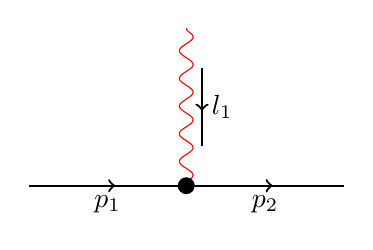
\begin{tikzpicture}[scale=1]
       \draw[photon](0,0)to(0,-2);
       \draw[nucleon, thick](-2,-2)to(0,-2);
       \draw[nucleon, thick](0,-2)to(2,-2);            
       \node[below] at (-1,-2) {$p_1$};
       \node[below] at (1,-2) {$p_2$};
       \node[right] at (0.2,-1) {$l_1$};
       \draw[nucleon, thick](0.2,-0.5)to(0.2,-1.5);
       \draw[fill] (0,-2) circle (0.1);
   \end{tikzpicture}
   \caption{Feynman rules for $ep\to ep\gamma$ up to $O(p^3)$}
\end{figure}

\begin{align}
   \begin{aligned}
       O(p^1):& -ie\gamma^{\mu}, \\
       O(p^2):& -ie (c_6+c_7)\gamma^{\mu} + \frac{ie(c_6+c_7)}{2m_N}(p_1+p_2)^{\mu},\\
       O(p^3):& \frac{ie(d_6+2d_7)(p_1-p_2)^2}{m_N}(p_1+p_2)^{\mu}.
       \label{feyrules}
   \end{aligned}
\end{align}




\subsection{Feynman Diagram Calculations}

The Feynman diagrams for the $ep\to ep\gamma$ process can be broadly divided into two categories: a photon radiating from the lepton (electron) leg, and a photon radiating from the hadron (proton) leg. These two categories can be further subdivided into three distinct diagram structures, as shown in Figure \ref{fig2.fushe}.



\begin{figure}[H]
    \centering
    \subfigure[]{
    \begin{minipage}[t]{0.3\textwidth}
        \centering
        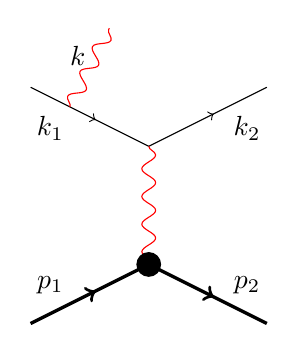
\begin{tikzpicture}[scale=0.5]
            \draw[nucleon](-3,1.5)to(0,0);
            \draw[nucleon](0,0)to(3,1.5);
            \draw[nucleon, very thick](-3,-4.5)to(0,-3);
            \draw[nucleon, very thick](0,-3)to(3,-4.5);
            \draw[photon](0,0)to(0,-3);
            \draw[photon](-2,1)to(-1,3);
            \draw[fill] (0,-3) circle (0.3);
            \node[above] at (-1.8,1.8) {$k$};
            \node[below] at (-2.5,1) {$k_1$};
            \node[below] at (2.5,1) {$k_2$};
            \node[above] at (-2.5,-4) {$p_1$};
            \node[above] at (2.5,-4) {$p_2$};
            
        \end{tikzpicture}
        \label{fig2.eii}
    \end{minipage}}
    \subfigure[]{
    \begin{minipage}[t]{0.3\textwidth}
        \centering
        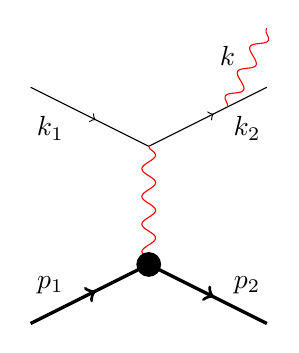
\begin{tikzpicture}[scale=0.5]
            \draw[nucleon](-3,1.5)to(0,0);
            \draw[nucleon](0,0)to(3,1.5);
            \draw[nucleon, very thick](-3,-4.5)to(0,-3);
            \draw[nucleon, very thick](0,-3)to(3,-4.5);
            \draw[photon](2,1)to(3,3);
            \draw[photon](0,0)to(0,-3);
            \draw[fill] (0,-3) circle (0.3);
            \node[above] at (2,1.8) {$k$};
            \node[below] at (-2.5,1) {$k_1$};
            \node[below] at (2.5,1) {$k_2$};
            \node[above] at (-2.5,-4) {$p_1$};
            \node[above] at (2.5,-4) {$p_2$};
            \label{fig2.eff}
        \end{tikzpicture}
    \end{minipage}}
    \centering
    \subfigure[]{
    \begin{minipage}[t]{0.3\textwidth}
        \centering
        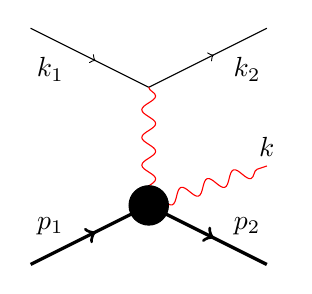
\begin{tikzpicture}[scale=0.5]
            \draw[nucleon](-3,1.5)to(0,0);
            \draw[nucleon](0,0)to(3,1.5);
            \draw[nucleon, very thick](-3,-4.5)to(0,-3);
            \draw[nucleon, very thick](0,-3)to(3,-4.5);
            \draw[photon](0,0)to(0,-3);
            \draw[photon](0,-3)to(3,-2);
            \draw[fill] (0,-3) circle (0.5);
            \node[above] at (3,-2) {$k$};
            \node[below] at (-2.5,1) {$k_1$};
            \node[below] at (2.5,1) {$k_2$};
            \node[above] at (-2.5,-4) {$p_1$};
            \node[above] at (2.5,-4) {$p_2$};

        \end{tikzpicture}
        \label{fig2.p}
    \end{minipage}}
    \caption{Bremsstrahlung Processes}
    \label{fig2.fushe}
\end{figure}

Figures \ref{fig2.eii} and \ref{fig2.eff} depict the electron bremsstrahlung process, whose amplitudes are primarily described by QED theory, while the proton part is simplified to a "black box" described by form factors. Figure \ref{fig2.p} describes a virtual Compton scattering process, where a virtual photon interacts with a proton and radiates a real photon. The amplitudes of these three diagrams must be calculated separately and summed to obtain the total scattering amplitude.

For diagrams where the photon radiates from the lepton leg, the amplitude can be decomposed into a leptonic part and a hadronic part. The amplitude $ \mathcal{M}_a,\mathcal{M}_b$ for Figure \ref{fig2.eii} and \ref{fig2.eff} can be written as :   
\begin{align}
    \begin{aligned}
    \mathcal{M}_{a}&=\bar{u}(k_2,m_e)(-ie\gamma^{\mu})\frac{i(\slashed{k}_1-\slashed{k}+m_e)}{(k_1-k)^2-m_e^2}(-ie\gamma^{\nu})u(k_1,m_e)\frac{-i}{l_1^2}\bar{u}(p_2,m_N)\Gamma_{\mu}u(p_1,m_N)\epsilon_{\nu}^{*}\\
    &=\frac{e^2}{l_1^2}\frac{-1}{(k_1-k)^2-m_e^2}\bar{u}(k_1,m_e)\gamma^{\mu}(\slashed{k}_1-\slashed{k}+m_e)\gamma^{\nu}u(k_1,m_e)\bar{u}(p_2,m_N)\Gamma_{\mu}u(p_2,m_N)\epsilon_{\nu}^{*},\\
     \mathcal{M}_{b}&=\bar{u}(k_2,m_e)(-ie\gamma^{\nu})\frac{i(\slashed{k}+\slashed{k}_2+m_e)}{(k+k_2)^2-m_e^2}(-ie\gamma^{\mu})u(k_1,m_e)\frac{-i}{l_1^2}\bar{u}(p_1,m_N)\Gamma_{\mu}u(p_2,m_N)\epsilon_{\nu}^{*}\\
        &=\frac{e^2}{l_1^2}\frac{-1}{(k+k_2)^2-m_e^2}\bar{u}(k_1,m_e)\gamma^{\nu}(\slashed{k}+\slashed{k}_2+m_e)\gamma^{\mu}u(k_1,m_e)\bar{u}(p_1,m_N)\Gamma_{\mu}u(p_1,m_N)\epsilon_{\nu}^{*}.
    \end{aligned}
\end{align}

In the expressions above, the hadronic part is described by $\Gamma_{\mu}$, which is a complex structure containing nucleon form factors. It can generally be decomposed into the Dirac form factor $F_1^N(Q^2)$ and the Pauli form factor $F_2^N(Q^2)$: 
\begin{align}
    \Gamma^{\mu}=F_1^N(Q^2)\gamma^{\mu}+i\frac{\sigma^{\mu\nu}q_{\nu}}{2m_N}F_2^N(Q^2).
\end{align}
where $Q=p_2-p_1$. These form factors summarize the influence of the proton's internal structure on electromagnetic interactions, rather than behaving as a simple point particle.

For the virtual Compton scattering process in Figure \ref{fig2.p}, its amplitude $\mathcal{M}_{c}$ can be written in the following form:
\begin{align}
    \begin{aligned}
        \mathcal{M}_{c}&=\bar{u}(k_2,m_e)(-ie\gamma_{\mu})u(k_1,m_e)\frac{-i}{l_1^2}\bar{u}(p_2,m_N)(\Gamma_1^{\mu\nu}+\Gamma_2^{\nu\mu})u(p_1,m_N)\epsilon_{\nu}^{*}\\
        &=\frac{-1}{l_1^2}e\bar{u}(k_2,m_e)\gamma_{\mu}u(k_1,m_e)\bar{u}(p_2,m_N)(\Gamma_1^{\mu\nu}+\Gamma_2^{\nu\mu})u(p_1,m_N)\epsilon_{\nu}^{*}.
    \end{aligned}
\end{align}
where $\Gamma_{1}^{\mu\nu}$ and $\Gamma_{2}^{\nu\mu}$ represent the complex hadronic part where a virtual photon interacts with the proton and radiates a real photon. For simplification, this hadronic part can be rearranged and defined as the virtual Compton scattering amplitude $M_{1}^{\mu\nu}$, with the expression $\overline{u}(p_2,m_N)(\Gamma_{1}^{\mu\nu}+\Gamma_{2}^{\nu\mu})u(p_1,m_N)\epsilon_{\nu}^{*}\equiv M_{1}^{\mu\nu}\epsilon_{\nu}^{*}$.
For ease of calculation, the hadronic amplitude $M_{1}^{\mu\nu}$ is usually decomposed according to its Lorentz structure :
$$M_{1}^{\mu\nu}=\sum_{i}\bar{u}(p_2,m_N)A_{i}\Gamma_{i}^{\mu\nu}u(p_1,m_N),$$
where $\Gamma_{i}^{\mu\nu}$ is a combination of 26 fundamental Lorentz structures, such as $g^{\mu\nu}$, $\gamma^{\mu}\gamma^{\nu}$, and various tensors formed from the momenta $k, p_1, p_2$, etc., as shown in Table \ref{table_amp}. This decomposition is a common method for handling complex hadronic amplitudes, transforming the problem of calculating the amplitude into one of solving for a series of scalar coefficients $A_i$.

For virtual Compton scattering, calculating at tree level up to $O(p^3)$ order, we obtain the following results (where $p$ denotes that the fermion is a proton). Let the four-momentum of the virtual photon be $l_1 = k + p_2 - p_1$:




\begin{figure}[H]
    % \renewcommand{\figurename}{图}
    \centering
    \begin{minipage}[t]{0.3\textwidth}
        \centering
        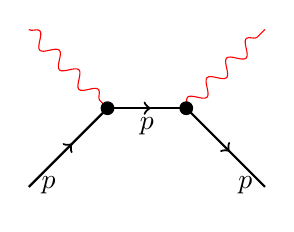
\begin{tikzpicture}[scale=0.5]
            \draw[photon](-3,2)to(-1,0);
            \draw[nucleon, thick](-1,0)to(1,0);
            \draw[photon](1,0)to(3,2);
            \draw[nucleon, thick](-3,-2)to(-1,0);
            \draw[nucleon, thick](1,0)to(3,-2);
            \node[below] at(-2.5,-1.5) {$p$};
            \node[below] at(2.5,-1.5) {$p$};
            \node[below] at(0,0) {$p$};
            \fill (-1,0) circle (5pt);
            \fill (1,0) circle (5pt);
        \end{tikzpicture}
        \caption*{(1)}
    \end{minipage}
    \begin{minipage}[t]{0.3\textwidth}
        \centering
        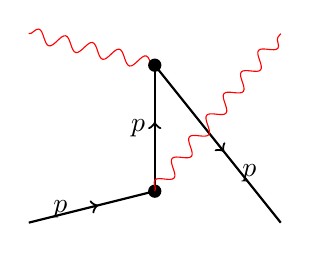
\begin{tikzpicture}[scale=0.8]
            \draw[photon](-2,0.5) to(0,0);
            \draw[nucleon, thick](-2,-2.5)to(0,-2);
            \fill (0,0) circle (3pt);
            \fill (0,-2) circle (3pt);
            \draw[nucleon, thick](0,-2) to (0,0);
            \draw[nucleon, thick](0,0) to (2,-2.5);
            \draw[photon](0,-2) to (2,0.5);
            \node[below] at(-1.5,-2) {$p$};
            \node[left] at(0,-1) {$p$};
            \node[above] at(1.5,-2) {$p$};
        \end{tikzpicture}
        \caption*{(2)}
    \end{minipage}
    \begin{minipage}[t]{0.3\textwidth}
        \centering
        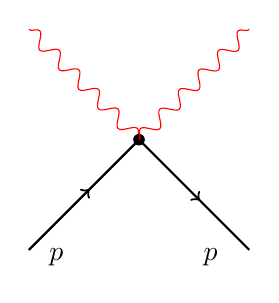
\begin{tikzpicture}[scale=0.7]
            \draw[photon](-2,2) to(0,0);
            \draw[nucleon, thick](-2,-2)to(0,0);
            \fill (0,0) circle (3pt);
            \draw[nucleon, thick](0,0) to (2,-2);
            \draw[photon](0,0) to (2,2);
            \node[below] at(-1.5,-1.8) {$p$};
            \node[below] at(1.3,-1.8) {$p$};
        \end{tikzpicture}
        \caption*{(3)}
    \end{minipage}
    \caption{Virtual Compton Scattering diagrams}
    \label{vcsdiagram}
\end{figure}

Using the derived Feynman rules \cref{feyrules}, we can easily obtain the amplitude for Figure \ref{vcsdiagram} as follows:
\begin{align}
    \begin{aligned}
        \mathcal{M}_1=&i\bar{u}(p_2,m_N)\cdot\Bigl(
            \frac{ie(c_6+c_7)\slashed{k}\slashed{\epsilon}^*(k)}{4m_N} - \frac{ie(c_6+c_7)\slashed{\epsilon}^*(k) \slashed{k}}{4m_N} +\frac{ie(d_6+2d_7)k^2 p_2\cdot \epsilon^*(k)}{m_N} -ie \slashed{\epsilon}^*(k)
         \Bigr)\\
         &\frac{(\slashed{p}_2+\slashed{k})+m}{(k+p_2)^2-m^2}\cdot
        \Bigl(
           -\frac{ie (c_6+c_7)\slashed{l}_1 \slashed{\epsilon}(l_1)}{4m_N} +\frac{ie(c_6+c_7)\slashed{\epsilon}(l_1)\slashed{l}_1}{4m_N} - ie \slashed{\epsilon}(l_1)+ \\
           &\frac{ie(d_6+2d_7) l_1 \cdot \epsilon(l_1)(- l_1 \cdot(k+p_2+p_1))}{2m_N} -\frac{ie(d_6+2d_7)l_1^2(-\epsilon(l_1)\cdot(k+p_2+p_1))}{2m_N}
        \Bigr)u(p_1,m_N),
    \end{aligned}
\end{align}
\begin{align}
    \begin{aligned}
        \mathcal{M}_2=&i\bar{u}(p_2,m_N)\Bigl(
           -\frac{ie (c_6+c_7)\slashed{l}_1 \slashed{\epsilon}(l_1)}{4m_N} +\frac{ie(c_6+c_7)\slashed{\epsilon}(l_1)\slashed{l}_1}{4m_N} - ie \slashed{\epsilon}(l_1)\\
           &-\frac{ie(d_6+2d_7)l_1\cdot \epsilon(l_1)(l_1\cdot(p_1+p_2-k))}{2m_N} +\frac{ie(d_6+2d_7)l_1^2(\epsilon(l_1)\cdot(p_1+p_2-k))}{2m_N}
        \Bigr)\cdot
         \frac{(\slashed{p}_1-\slashed{k})+m}{(k-p_1)^2-m^2}\cdot\\
        &\Bigl(
           \frac{ie(c_6+c_7)\slashed{k}\slashed{\epsilon}^*(k)}{4m_N} - \frac{ie(c_6+c_7)\slashed{\epsilon}^*(k) \slashed{k}}{4m_N} +\frac{ie(d_6+d_7)k^2(p_1\cdot \epsilon^*(k))}{m_N}-ie \slashed{\epsilon}^*(k)
        \Bigr)u(p_1,m_N),
    \end{aligned}
\end{align}

\begin{align}
    \begin{aligned}
        \mathcal{M}_3=\bar{u}(p_2,m_N)  \frac{i e^2 (d_6+2d_7)}{m_N}([l_1\cdot \epsilon(l_1)][l_1\cdot\epsilon^*(k)]-k^2[\epsilon(l_1)\cdot \epsilon^*(k)]-l_1^2[\epsilon(l_1)\cdot \epsilon^*(k)])u(p_1,m_N).
    \end{aligned}
\end{align}



These initial expressions incorporate higher-order terms that require truncation in accordance with the chiral power counting scheme outlined in \cite{scherer2005}. As explicitly noted in the document, given that the vertices are of order \(O(p^3)\) at most, the resulting amplitude can extend up to \(O(p^5)\). Since the amplitude is calculated up to \(O(p^3)\) in this work, its squared magnitude consequently reaches up to \(O(p^6)\). To ensure theoretical consistency throughout the calculation, all terms in the amplitude beyond the \(O(p^3)\) order must be systematically eliminated. Note that only terms in the amplitude beyond \(O(p^3)\) are discarded here; terms appearing in \(|\mathcal{M}|^2\) at orders higher than \(O(p^3)\) have not been removed.


To facilitate calculations within the software, we first need to define the five Mandelstem variables as follows:
\begin{align}
    \begin{aligned}
        s=(k_1+&p_1)^2,\quad s_1=(k+p_2)^2,\quad s_2=(k+k_2)^2,\\
        &t_1=(k-p_1)^2,\quad t_2=(p_1-p_2)^2.
    \end{aligned}
\end{align}

Based on the definition of the Mandelstem variables, the scattering amplitude can be systematically simplified. After truncation and rearrangement, the results for each order of the amplitude are as follows: 
\begin{table}[H]
    \centering
    \resizebox{\linewidth}{!}{
        \renewcommand{\arraystretch}{2} 
        {\Huge
    \begin{tabular}{ccccc}
      \hline
      \rowcolor{green!40}
            & $\gamma^{\mu}\gamma^{\nu}$ & $\gamma^{\mu}\gamma^{\nu}\slashed{k}$ & $k^{\mu}\gamma^{\nu}$ &$k^{\mu}\gamma^{\nu}\slashed{k}$\\
      \hline
      $\mathcal{M}^{(1)\mu\nu}$& $0$ & $\frac{ie^2}{m_N^2-s_1}+\frac{ie^2}{m_N^2-t_1}$ & $0$ &$-\frac{-2ie^2}{m_N^2-s_1}$\\
      \hline
      $\mathcal{M}^{(2)\mu\nu}$& 0 & $\frac{2m_N A}{m_N^2-s_1}+\frac{2A}{m_N^2-t_1}$& $-2A$ &$-\frac{4A}{m_N^2-s_1}$\\
      \hline
      $\mathcal{M}^{(3)\mu\nu}$& 0&$\frac{B(3m_N^2+s_1)}{4(m_N^2-s_1)}+\frac{B(3m_N^2+t_1)}{4(m_N^2-t_1)}$ &$\frac{C(2m_N^2-s_1-t_1-t_2)}{m_N}-B$ &$-\frac{B(3m_N^2+s_1)}{2(m_N^3-m_N t_1)}$\\
      \hline
      \rowcolor{green!40}
      & $p_1^{\mu}\gamma^{\nu}$ & $p_1^{\mu}\gamma^{\nu}\slashed{k}$ & $p_2^{\mu}\gamma^{\nu}$ &$p_2^{\mu}\gamma^{\nu}\slashed{k}$\\
      \hline
      $\mathcal{M}^{(1)\mu\nu}$& $\frac{2ie^2}{m_N^2-s_1}$ & 0 & 0 &0\\
      \hline
      $\mathcal{M}^{(2)\mu\nu}$& $\frac{4m_N A}{m_N^2-s_1}$ & $-\frac{A}{2(m_N^2-s_1)}+\frac{A}{2(m_N^2-t_1)}$ & 0 &$-\frac{A}{2(m_N^2-s_1)}-\frac{A}{2(m_N^2-t_1)}$\\
      \hline
      $\mathcal{M}^{(3)\mu\nu}$& $-\frac{B(7m_N^2+s_1)}{4(m_N^2-s_1)}-\frac{1}{4}B$& $\frac{C(m_N^2-t_1-t_2)-Bm_N^2}{2(m_N^3-m_N s_1)}+\frac{Bm_N^2-C(m_N^2- s_1-t_2)}{2(m_N^3-m_N t_1)}$&$\frac{1}{2}B$ &$\frac{C(3m_N^2-2s_1-t_1-t_2)-Bm_N^2}{2(m_N^3-m_N s_1)}+\frac{C(m_N^2-s_1-t_2)-Bm_N^2}{2(m_N^3-m_N t_1)}$\\
      \hline
      \rowcolor{green!40}
      & $g^{\mu\nu}$ & $g^{\mu\nu}\slashed{k}$ & $p_1^{\nu}\gamma^{\mu}$ &$p_1^{\nu}\gamma^{\mu}\slashed{k}$\\
      \hline
      $\mathcal{M}^{(1)\mu\nu}$& 0& 0 & $\frac{2ie^2}{m_N^2-t_1}$ &0\\
      \hline
      $\mathcal{M}^{(2)\mu\nu}$& 0 & $-\frac{A}{2(m_N^2-s_1)}-\frac{A}{2(m_N^2-t_1)}$ & $\frac{m_N A}{m_N^2-t_1}$&$\frac{A}{m_N^2-t_1}$\\
      \hline
      $\mathcal{M}^{(3)\mu\nu}$& $\frac{1}{2}B$ & $\frac{C(m_N^2-t_1-t_2)-Bm_N^2}{2(m_N^3-m_N s_1)}+\frac{C(3m_N^2-s_1-2t_1-t_2)-Bm_N^2}{(2m_N^3-m_N t_1)}$ & 0 &$\frac{C(m_N^2-t_1-t_2)}{m_N^3-m_N s_1}+\frac{B m_N}{m_N^2-t_1}$\\
      \hline
      \rowcolor{green!40}
      & $k^{\mu}p_1^{\nu}$ & $k^{\mu}p_1^{\nu}\slashed{k}$ & $p_1^{\mu}p_1^{\nu}$ &$p_1^{\mu}p_1^{\nu}\slashed{k}$\\
      \hline
      $\mathcal{M}^{(1)\mu\nu}$& $\frac{2ie^2}{m_N^2-s_1}$ & 0 & 0 &0\\
      \hline
      $\mathcal{M}^{(2)\mu\nu}$& $\frac{m_N A}{m_N^2-s_1}$ & $\frac{A}{m_N^2-s_1}$& $-\frac{A}{m_N^2-t_1}$ &0\\
      \hline
      $\mathcal{M}^{(3)\mu\nu}$&  0&  $\frac{B m_N}{m_N^2-s_1}$& $\frac{C}{m_N}+\frac{C(m_N^2-s_1-t_2)}{m_N^3-m_N t_1}$ &$\frac{C(m_N^2-t_1-t_2)}{m_N^3-m_N s_1}-\frac{B}{2(m_N^2-t_1)}$ \\
      \hline
      \rowcolor{green!40}
      & $p_2^{\mu}p_1^{\nu}$ & $p_2^{\mu}p_1^{\nu}\slashed{k}$ & $p_2^{\nu}\gamma^{\mu}$ &$p_2^{\nu}\gamma^{\mu}\slashed{k}$\\
      \hline
      $\mathcal{M}^{(1)\mu\nu}$& 0 & 0 & 0 &0\\
      \hline
      $\mathcal{M}^{(2)\mu\nu}$& $-\frac{A}{m_N^2-s_1}$ & 0 & $\frac{A}{m_N^2-t_1}$&0\\
      \hline
      $\mathcal{M}^{(3)\mu\nu}$& $\frac{C}{m_N}+\frac{C(m_N^2-t_1-t_2)}{m_N^3-m_N s_1}$ & $\frac{B}{2(m_N^2-s_1)}$ & $-\frac{C}{m_N}-\frac{C(m_N^2-s_1-t_2)}{m_N^3-m_N t_1}$ &$\frac{B}{2(m_N^2-t_1)}$\\
      \hline
      \rowcolor{green!40}
       & $k^{\mu}p_2^{\nu}$ &$k^{\mu}p_2^{\nu}\slashed{k}$& $p_1^{\mu}p_2^{\nu}$& $p_1^{\mu}p_2^{\nu}\slashed{k}$\\
      \hline
      $\mathcal{M}^{(1)\mu\nu}$& 0 & 0 & 0 &0\\
      \hline
      $\mathcal{M}^{(2)\mu\nu}$& $-\frac{3A}{m_N^2-s_1}$ & 0 & $-\frac{A}{m_N^2-s_1}$ &0\\
      \hline
      $\mathcal{M}^{(3)\mu\nu}$& $\frac{C}{m_N}+\frac{C(m_N^2-t_1-t_2)}{m_N^3-m_N s_1}-\frac{2 B m_N}{m_N^2-s_1}$ & $\frac{C}{2(m_N^2-s_1)}$ & $-\frac{C}{m_N}+\frac{C(3m_N^2-2s_1-t_1-t_2)}{m_N^3-m_N s_1}$ &$\frac{B}{2(m_N^2-s_1)}$\\
      \hline
      \rowcolor{green!40}
       & $p_2^{\mu}p_2^{\nu}$ &$p_2^{\mu}p_2^{\nu}\slashed{k}$&&\\
      \hline
      $\mathcal{M}^{(1)\mu\nu}$& 0 & 0 &  &\\
      \hline
      $\mathcal{M}^{(2)\mu\nu}$& $-\frac{A}{m_N^2-t_1}$ & 0 &  &\\
      \hline
      $\mathcal{M}^{(3)\mu\nu}$& $-\frac{C}{m_N}+\frac{C(3m_N^2-s_1-2t_1-t_2)}{m_N^3-m_N t_1}$ & $-\frac{B}{2(m_N^2-t_1)}$ &  &\\
      \hline
    \end{tabular}}
    }
    \caption{Virtual Compton Scattering amplitudes, where $A=ie^2(c_6+c_7)$, $B=ie^2(c_6+c_7)^2$, and $C=ie^2(d_6+2d_7)$.}
    \label{table_amp}
  \end{table}
  
  It is important to note a key detail here, which is the use of mass in the proton propagator. The $c_1$ term in the Lagrangian introduces a mass correction, i.e., $m\to m_2=m - 4c_1 M^2$ . However, $m_2-m_N \sim O(p^3)$, and this mass difference only appears in $O(p^3)$ loop diagram calculations. Since this is a tree diagram calculation, the propagator mass can be directly replaced with the true nucleon mass $m_N$.For example, the original form of the \( \gamma^{\mu} \gamma^{\nu} \slashed{k} \) term in \( M^{(1)\mu\nu} \) is \( \frac{ie^2}{m_2^2 - s_1} +\frac{ie^2}{m_2^2-t_1}\), but after applying the substitutions, it is expressed as shown in the table.
  
\subsection{Kinematics and Formalism}

In the context of the $e(k_1)+p(p_1) \rightarrow e(k_2)+p(p_2)+\gamma(k)$ process, experimental data is typically expressed in terms of a set of standard variables, including the virtuality $Q^2$, the Bjorken scaling variable $x_B$, and the momentum transfer $t$. These are defined as follows \cite{defurne2015e00}:
\begin{align}
Q^2=-q^2=-(k_1-k_2)^2,\quad x_B=Q^2/(2q\cdot p_1),\quad t=(p_2-p_1)^2.
\end{align}

Additionally, the covariant azimuthal angle $\phi$ is defined by Eq. (\ref{cosphi}) \cite{phiAngle}. The schematic diagram of the $\phi$ angle is shown in Fig \ref{fig:axes}, which is defined as the angle between the lepton plane and the hadron plane\cite{Boer_1998,Mulders_1996}. The lepton plane is formed by the incident and scattered leptons, whereas the hadron plane is defined by the momentum transfer vector—given by the difference between the incident and scattered lepton momenta—and the outgoing proton.


\begin{figure}[htbp]
    \centering
    \includegraphics[width=\textwidth]{./e100axes.pdf}
    \caption{Definition of azimuthal angles for the $ep\to ep \gamma$ process in the target rest frame.}
    \label{fig:axes}
\end{figure}

\begin{align}
{\rm cos} \phi = -\frac{g^{\mu\nu}_{\bot}k_{1 \mu}p_{2\nu}}{|k_{1\bot}||p_{2\bot}|},  \quad
{\rm sin} \phi = -\frac{\varepsilon^{\mu\nu}_{\bot}k_{1\mu}p_{2\nu}}{|k_{1\bot}||p_{2\bot}|},
\label{cosphi}
\end{align}
where
\begin{align}
|k_{1\bot}|=&\sqrt{-g^{\mu\nu}_{\bot}k_{1\mu} k_{1\nu}},\quad |p_{2\bot}|=\sqrt{-g^{\mu\nu}_{\bot}p_{2\mu} p_{2\nu}},\\
g^{\mu\nu}_\bot =&g^{\mu\nu} - \frac{q^{\mu}p_1^{\nu}+p_1^{\mu}q^{\nu}}{p_1\cdot q(1+\gamma^2)} + \frac{\gamma^2}{1+\gamma^2}(\frac{q^{\mu}q^{\nu}}{-q^2}-\frac{p_1^\mu p_1^\nu}{m_N^2}),\\
\varepsilon^{\rho\sigma}_{\bot}=&\varepsilon^{\mu\nu\rho\sigma}\frac{p_{1\mu} q_\nu}{p_1\cdot q\sqrt{1+\gamma^2}}.
\end{align}
where $\gamma=2x_B m_N/Q,q=k_1-k_2$.



The differential scattering cross-section is a crucial quantity that directly links theoretical calculations to experimental measurements. The complete differential scattering cross-section for this process is given by \cite{defurne2015e00}:
\begin{align}
\frac{d^5\sigma}{dQ^2 dx_B dt d\phi d\phi_e}=\frac{\alpha_{QED}^3}{16\pi^2(s_e-M^2)^2 x_B}\frac{1}{\sqrt{1+\varepsilon^2}}\frac{1}{e^6}|\mathcal{M}|^2,
\end{align}
where 
\begin{align}
\varepsilon^2 = 4M^2 x_B^2/Q^2, \quad s_e=(k_1+p_1)^2.
\end{align}

Due to the rotational symmetry of the scattered lepton around the incident axis in the laboratory frame, the scattering result is independent of the angle $\phi_e$. It is therefore common practice to integrate over the $\phi_e$ angle, which simplifies the expression by a factor of $2\pi$, resulting in the following differential scattering cross-section:
\begin{align}
    \frac{d^4\sigma}{dQ^2 dx_B dt d\phi }=\frac{\alpha_{QED}^3}{8\pi(s_e-M^2)^2 x_B}\frac{1}{\sqrt{1+\varepsilon^2}}\frac{1}{e^6}|\mathcal{M}|^2.
\end{align}


For the $ep \to e p \gamma$ process, the amplitude $\mathcal{M}$ can be decomposed into the sum of the amplitude from the lepton leg radiation $\mathcal{M}_e$ and the amplitude from the nucleon leg radiation $\mathcal{M}_p$, i.e., $\mathcal{M} = \mathcal{M}_e + \mathcal{M}_p$.
Furthermore, the amplitude can be partitioned according to its chiral order:
\begin{align}
    \mathcal{M} = \mathcal{M}^{(1)} + \mathcal{M}^{(2)} + \dots = (\mathcal{M}^{(1)}_{e} + \mathcal{M}^{(2)}_{e} + \dots) + (\mathcal{M}^{(1)}_{p} + \mathcal{M}^{(2)}_{p} + \dots).
\end{align}

When calculating the squared amplitude, interference terms between different parts also are considered. For example, for the $O(p^{1})$ order, the squared amplitude is :
\begin{align}
    |\mathcal{M}^{(1)}|^2 = |\mathcal{M}^{(1)}_{e}|^2 + |\mathcal{M}^{(1)}_{p}|^2 + 2\Re(\mathcal{M}^{(1)}_{e} \mathcal{M}^{*(1)}_{p}).
\end{align}











\section{Comparison with Experiments}
To compare experimental results with theoretical calculations, we need to ensure the variables are consistent. We can easily convert $s,s_1,s_2,t_1,t_2$ into functions of $Q^2,x_B,t,\phi$ and $E_k$, where $E_k$ is the energy of the incident lepton in the lab frame.
\begin{align}
s =&m_e^2 + m_N^2 + 2m_N E_k,\\
s_1=&-\frac{-Q^2-m_N^2 x_B+Q^2 x_B}{x_B},\\
t_1=&-\frac{Q^2-m_N^2 x_B+t x_B}{x_B},\\
t_2=&t.
\end{align}
As for $s_2$, its numerical relationship with $Q^2,x_B,t,\phi, E_k$ can be easily derived.

The experimental data has been summarized in Tables 7, 8, 12, and 13 of \cite{defurne2015e00}, with each table corresponding to a different kinematic range.
Firstly, we adopt the parameter values from Table~2 in Ref.~\cite{fuchs2004electromagnetic}, namely $c_6=1.34, c_7=-0.15, d_6=-0.70$, and $d_7=-0.49$. 
It should be noted that a parameter transformation is required according to footnote~\ref{lecs_footnote}. 
The results are shown in \Cref{fig:table7_plot,fig:table8_plot,fig:table12_plot,fig:table13_plot}: it can be observed that the theoretical calculations do not agree well with the experimental data. 
Specifically, the $O(p^3)$ results are significantly larger than those at $O(p^2)$, and the $O(p^2)$ results are also considerably higher than the $O(p^1)$ order. 
\begin{figure}[htbp]
    \centering
    \includegraphics[width=\textwidth]{./table7_plot.pdf} % 请根据实际文件名和路径调整
    \caption{Comparison between the calculated results and experimental data from Table 7 in Ref.~\cite{defurne2015e00}}
    \label{fig:table7_plot}
\end{figure}
\begin{figure}[htbp]
    \centering
    \includegraphics[width=\textwidth]{./table8_plot.pdf} % 请根据实际文件名和路径调整
    \caption{Comparison between the calculated results and experimental data from Table 8 in Ref.~\cite{defurne2015e00}}
    \label{fig:table8_plot}
\end{figure}
\begin{figure}[htbp]
    \centering
    \includegraphics[width=\textwidth]{./table12_plot.pdf} % 请根据实际文件名和路径调整
    \caption{Comparison between the calculated results and experimental data from Table 12 in Ref.~\cite{defurne2015e00}}
    \label{fig:table12_plot}
\end{figure}
\begin{figure}[htbp]
    \centering
    \includegraphics[width=\textwidth]{./table13_plot.pdf} % 请根据实际文件名和路径调整
    \caption{Comparison between the calculated results and experimental data from Table 13 in Ref.~\cite{defurne2015e00}}
    \label{fig:table13_plot}
\end{figure}









We attribute this discrepancy primarily to the large value of $Q^2$. 
Although $-t \in [-0.372, -0.171] \, \text{GeV}^2$, the value of $Q^2$ has exceeded the validity region of Chiral Perturbation Theory ($\chi PT$), leading to the poor agreement. 

Subsequently, we attempted to fit the Low-Energy Constants (LECs) based on the experimental data. 
For the $O(p^2)$ fit, the results remain unsatisfactory, which is not unexpected since $c_6+c_7$ is the sole variable at this order; achieving a high-quality fit with only one parameter is inherently difficult. 
However, at $O(p^3)$, despite the addition of effectively only one more parameter combination $d_6+2d_7$, the fitting results show a surprising improvement. 







Here, we present the individual fitting results for each table, as well as the overall fitting results when all tables are combined.
\begin{figure}[htbp]
    \centering
    \includegraphics[width=\textwidth]{./table7_fit_plot.pdf} % 请根据实际文件名和路径调整
    \caption{Fit Results for Table 7 data in \cite{defurne2015e00}}
    \label{fig:table7_fit}
\end{figure}

\begin{table}[htbp]
\centering
\caption{Fitted parameters $\alpha_1=c_6+c_7$ and $\alpha_2=d_6+2d_7$, and $\chi^2/dof$ values for different orders for Table 7 data in \cite{defurne2015e00}}
\label{table7_results}
\begin{tabular}{l c c}
\toprule
& \textbf{$O(p^2)$ } & \textbf{$O(p^3)$ } \\
\midrule
% 使用 array 环境实现垂直居中
$\begin{array}{@{}l@{}}
\alpha_1 = c_6 + c_7, \\
\alpha_2 = d_6 + 2d_7
\end{array}$ 
& 
$\alpha_1 = -0.2149 \pm 0.0720$ 
& 
$\begin{aligned}
\alpha_1 &= 0.2867 \pm 0.0161, \\
\alpha_2 &= -1.2580 \pm 0.0172
\end{aligned}$ \\
\midrule
$\chi^2/\mathrm{dof}$ & 61.13 & 3.54 \\
\bottomrule
\end{tabular}
\end{table}

\begin{figure}[H]
    \centering
    \includegraphics[width=\textwidth]{./table8_fit_plot.pdf} % 请根据实际文件名和路径调整
    \caption{Fit Results for Table 8 data in \cite{defurne2015e00}}
    \label{fig:table8_fit}
\end{figure}

\begin{table}[htbp]
\centering
\caption{Fitted parameters $\alpha_1=c_6+c_7$ and $\alpha_2=d_6+2d_7$, and $\chi^2/dof$ values for different orders for Table 8 data in \cite{defurne2015e00}}
\label{table8_results}
\begin{tabular}{l c c}
\toprule
& \textbf{$O(p^2)$ } & \textbf{$O(p^3)$ } \\
\midrule
% 使用 array 环境实现垂直居中
$\begin{array}{@{}l@{}}
\alpha_1 = c_6 + c_7, \\
\alpha_2 = d_6 + 2d_7
\end{array}$ 
& 
$\alpha_1 = -0.3437 \pm 0.0636$ 
& 
$\begin{aligned}
\alpha_1 &= 0.1089 \pm 0.0159, \\
\alpha_2 &= -1.1365 \pm 0.0172
\end{aligned}$ \\
\midrule
$\chi^2/\mathrm{dof}$ & 71.62 & 5.97 \\
\bottomrule
\end{tabular}
\end{table}

\begin{figure}[htbp]
    \centering
    \includegraphics[width=\textwidth]{./table12_fit_plot.pdf} % 请根据实际文件名和路径调整
    \caption{Fit Results for Table 12 data in \cite{defurne2015e00}}
    \label{fig:table12_fit}
\end{figure}

\begin{table}[htbp]
\centering
\caption{Fitted parameters $\alpha_1=c_6+c_7$ and $\alpha_2=d_6+2d_7$, and $\chi^2/dof$ values for different orders for Table 12 data in \cite{defurne2015e00}}
\label{table12_results}
\begin{tabular}{l c c}
\toprule
& \textbf{$O(p^2)$ } & \textbf{$O(p^3)$ } \\
\midrule
% 使用 array 环境实现垂直居中
$\begin{array}{@{}l@{}}
\alpha_1 = c_6 + c_7, \\
\alpha_2 = d_6 + 2d_7
\end{array}$ 
& 
$\alpha_1 = -0.2852 \pm 0.1147$ 
& 
$\begin{aligned}
\alpha_1 &= 0.1961 \pm 0.0212, \\
\alpha_2 &= -1.1721 \pm 0.0241
\end{aligned}$ \\
\midrule
$\chi^2/\mathrm{dof}$ & 30.95 & 1.38 \\
\bottomrule
\end{tabular}
\end{table}

\begin{figure}[htbp]
    \centering
    \includegraphics[width=\textwidth]{./table13_fit_plot.pdf} % 请根据实际文件名和路径调整
    \caption{Fit Results for Table 13 data in \cite{defurne2015e00}}
    \label{fig:table13_fit}
\end{figure}

\begin{table}[htbp]
\centering
\caption{Fitted parameters $\alpha_1=c_6+c_7$ and $\alpha_2=d_6+2d_7$, and $\chi^2/dof$ values for different orders for Table 13 data in \cite{defurne2015e00}}
\label{table13_results}
\begin{tabular}{l c c}
\toprule
& \textbf{$O(p^2)$ } & \textbf{$O(p^3)$ } \\
\midrule
% 使用 array 环境实现垂直居中
$\begin{array}{@{}l@{}}
\alpha_1 = c_6 + c_7, \\
\alpha_2 = d_6 + 2d_7
\end{array}$ 
& 
$\alpha_1 = -0.1577 \pm 0.0585$ 
& 
$\begin{aligned}
\alpha_1 &= 0.3158 \pm 0.0220, \\
\alpha_2 &= -1.2067 \pm 0.0234
\end{aligned}$ \\
\midrule
$\chi^2/\mathrm{dof}$ & 32.52 & 2.50 \\
\bottomrule
\end{tabular}
\end{table}

Finally, the result for the global fit of all data is shown in Fig.\ref{fig:tableAll_fit} :

\begin{figure}[H]
    \centering
    \includegraphics[width=\textwidth]{./all_fit.pdf} % 请根据实际文件名和路径调整
    \caption{Global fit results for all data in \cite{defurne2015e00}}
    \label{fig:tableAll_fit}
\end{figure}

\begin{table}[htbp]
\centering
\caption{Fitted parameters $\alpha_1=c_6+c_7$ and $\alpha_2=d_6+2d_7$, and $\chi^2/dof$ values for different orders for all data in \cite{defurne2015e00}}
\label{tableAll_results}
\begin{tabular}{l c c}
\toprule
& \textbf{$O(p^2)$ } & \textbf{$O(p^3)$ } \\
\midrule
% 使用 array 环境实现垂直居中
$\begin{array}{@{}l@{}}
\alpha_1 = c_6 + c_7, \\
\alpha_2 = d_6 + 2d_7
\end{array}$ 
& 
$\alpha_1 = -0.2786 \pm 0.0368$ 
& 
$\begin{aligned}
\alpha_1 &= 0.2114 \pm 0.0090, \\
\alpha_2 &= -1.1951 \pm 0.0098
\end{aligned}$ \\
\midrule
$\chi^2/\mathrm{dof}$ & 49.35 & 3.65 \\
\bottomrule
\end{tabular}
\end{table}

We determine $c_6+c_7=0.2114$ and $d_6+2d_7=-1.1951$ as our final results. 
A comparison reveals a significant discrepancy between our determined values and those reported in Ref.~\cite{fuchs2004electromagnetic}, where the corresponding converted parameters are $c_6+c_7=2.3747$ and $d_6+2d_7=-1.68$ (the values have been converted as detailed in footnote~\ref{lecs_footnote}). Regrettably, these results do not exhibit satisfactory agreement.



\section{Further Investigations}

As previously discussed, modern experimental precision has reached a level where the emission of photons can no longer be adequately addressed using the simple soft-photon approximation. 
We aim to further investigate the differential cross-section for the emission of hard photons. 
Furthermore, in ongoing $\mu p$ scattering experiments, the lepton mass can no longer be neglected. 
The differential cross-section without any approximations in the laboratory frame is given by:
\begin{align}
    \frac{\mathrm{d}\sigma}{\mathrm{d}E_{\gamma} \mathrm{d}\Omega_{\gamma} \mathrm{d}\Omega_{k_2}} 
    &= \frac{1}{(4\pi)^5} \frac{1}{m_N |\vec{k}_1|} 
    \sum_{E_{k_2}} \frac{E_\gamma |\vec{k}_2|^2 |\mathcal{M}|^2}{\left| A^{\prime} E_{k_2} - B^{\prime} |\vec{k}_2| \right|},
    \label{eq:diff_cross_section}
\end{align}
where $E_{\gamma}$ is the photon energy, $\Omega_{\gamma}$ is the solid angle of the emitted photon (characterized by the angle $\theta_{\gamma}$ with respect to the $z$-axis and the azimuthal angle $\phi_{\gamma}$), and $\Omega_{k_2}$ is the solid angle of the scattered lepton(same as $\Omega{\gamma}$). The kinematic variables $A^{\prime}$ and $B^{\prime}$ are defined as follows:
\begin{align}
    A^{\prime} &= |\vec{k}_1|{\rm cos}\theta_{k_2}-E_{\gamma}{\rm cos}\psi, \\
    {\rm cos}\psi &= {\rm cos}\theta_{k_2} {\rm cos}\theta_{\gamma}+{\rm sin} \theta_{k_2} {\rm sin }\theta_{\gamma} {\rm cos}\phi_{\gamma}\\
    B^{\prime} &= E_1 + m_N - E_{\gamma},
\end{align}


Using the formula derived above, we present a theoretical prediction for the hard photon differential cross-section, as illustrated in Fig.~\ref{fig:hard_photon_cross_section}. For this calculation, the low-energy constants (LECs) are adopted from Ref.~\cite{fuchs2004electromagnetic}.

\begin{figure}[htbp]
    \centering
    \includegraphics[width=0.9\linewidth]{lepton_proton_comparison_3mass_section.pdf} 
    \caption{Theoretical prediction of the differential cross-section for hard photon emission. The kinematic parameters are fixed at $\theta_{k^\prime} = 45^\circ$, $\theta_\gamma = 45^\circ$, $\phi_\gamma = 45^\circ$, and $E_\gamma = 0.1~\mathrm{GeV}$. The low-energy constants are taken from Ref.~\cite{fuchs2004electromagnetic}.}
    \label{fig:hard_photon_cross_section}
\end{figure}

From the figure, we can observe that the effect of the electron mass on the results is negligible. However, for $\mu p$ scattering, there are significant modifications to the differential cross-section. Furthermore, the figure indicates that while the Next-to-Leading Order (NLO) corrections maintain consistency with the Leading Order (LO) results, the Next-to-Next-to-Leading Order (NNLO) corrections exhibit different behavior as the incident energy increases. Specifically for $\mu p$ scattering, the scattering cross-section shifts from a decreasing to an increasing trend as the incident energy approaches 1 GeV. Combined with our previous experimental fitting results, this demonstrates that NNLO calculations are indispensable when considering bremsstrahlung corrections.


In addition, we also computed the differential cross-sections using the Low-Energy Constants (LECs) obtained from our global fit. Although there are some numerical discrepancies between these results and those derived using the parameters from Ref.~\cite{fuchs2004electromagnetic}, both calculations consistently demonstrate that the Next-to-Next-to-Leading Order (NNLO) corrections are indispensable. The comparison is illustrated in Fig.~\ref{fig:fitted_cross_section}.

\begin{figure}[htbp]
    \centering
    \includegraphics[width=0.9\linewidth]{lepton_proton_cross_section_me.pdf}
    \caption{Theoretical prediction of the differential cross-section using the fitted LECs from this work ($\alpha_1=0.2114, \alpha_2=-1.1951$). The kinematic parameters are the same as in Fig.~\ref{fig:hard_photon_cross_section}.}
    \label{fig:fitted_cross_section}
\end{figure}

\section{Conclusion}

This study presents a theoretical calculation of the scattering amplitude for the $ep\to ep\gamma$ process within the framework of Chiral Perturbation Theory (ChPT). We specifically focused on evaluating the tree-level Feynman diagrams up to $O(p^{3})$ that contribute to this reaction. The process is of significant importance as it provides valuable insights into the generalized polarizabilities of the nucleon, which are fundamental properties characterizing its response to electromagnetic fields.

Our calculations, based on the $O(p^{2})$ and $O(p^{3})$ nucleon-pion Lagrangians, aim to provide a theoretical prediction for the differential cross-section. By comparing our results with future experimental data, we aim to determine the values of the low-energy constants (LECs) and validate ChPT as an effective low-energy theory of QCD. The determination of LECs is crucial because they encode the complex dynamics of QCD at low energies, which are not predictable by the theory itself. By successfully fitting our calculations to experimental data, we can validate our theoretical approach and contribute to a more comprehensive understanding of strong interactions and nucleon structure.




\bibliographystyle{unsrt}
% \bibliographystyle{utphys}
\bibliography{ep}



\appendix









\end{document}

